\documentclass[twocolumn,11pt,a4paper]{article}

%% -----------------------------------------------------------------------
%%  Packages
%% -----------------------------------------------------------------------
\usepackage{amsmath,amssymb,amsthm}
\usepackage{mathtools}
\usepackage{microtype}
\usepackage{geometry}
\geometry{a4paper, top=2.2cm, bottom=2.2cm, left=1.8cm, right=1.8cm, columnsep=0.7cm}
\usepackage{hyperref}
\hypersetup{colorlinks=true,linkcolor=blue,citecolor=blue,urlcolor=blue}
\usepackage{cleveref}
\usepackage{booktabs}
\usepackage{array}
\usepackage{enumitem}
\usepackage{xcolor}
\usepackage{natbib}
\bibpunct{[}{]}{,}{n}{}{;}
\usepackage{titlesec}
\usepackage{abstract}
\usepackage{graphicx}
\usepackage{bm}

%% -----------------------------------------------------------------------
%%  Theorem environments
%% -----------------------------------------------------------------------
\newtheorem{theorem}{Theorem}[section]
\newtheorem{lemma}[theorem]{Lemma}
\newtheorem{proposition}[theorem]{Proposition}
\newtheorem{corollary}[theorem]{Corollary}
\newtheorem{definition}[theorem]{Definition}
\newtheorem{construction}[theorem]{Construction}
\newtheorem{example}[theorem]{Example}
\theoremstyle{remark}
\newtheorem{remark}[theorem]{Remark}

%% -----------------------------------------------------------------------
%%  Mathematical macros
%% -----------------------------------------------------------------------
\newcommand{\R}{\mathbb{R}}
\newcommand{\N}{\mathbb{N}}
\newcommand{\one}{\mathbf{1}}
\newcommand{\bw}{\mathbf{w}}
\newcommand{\bmu}{\bm{\mu}}
\newcommand{\Dm}{\Delta_m}
\newcommand{\Ld}{L^\dagger}
\newcommand{\lam}[1]{\lambda_{#1}}
\newcommand{\kap}{\kappa}
\newcommand{\sigtwo}{\sigma^2}
\newcommand{\norm}[1]{\left\lVert #1 \right\rVert_2}
\newcommand{\inner}[2]{\langle #1,\, #2 \rangle}
\newcommand{\Proj}{\Pi_\Delta}
\newcommand{\T}{\mathcal{T}}

%% -----------------------------------------------------------------------
%%  Title
%% -----------------------------------------------------------------------
\title{\textbf{Optimal Exchange-Traded Fund Construction\\
via Banach Fixed-Point Theory:\\
Portfolio Equilibrium, Risk, and\\
Composition-Inflation Execution}}

\author{
Kundai Farai Sachikonye\\
AIMe Registry for Artificial Intelligence\\
Experimental Bioinformatics\\
Maximus-von-Imhof-Forum 3\\
85354 Freising, Germany\\
\texttt{kundai.sachikonye@bitspark.com}
}

\date{\today}

\begin{document}

\maketitle

%% -----------------------------------------------------------------------
%%  Abstract
%% -----------------------------------------------------------------------
\begin{abstract}
\noindent
We develop a rigorous mathematical framework for exchange-traded fund (ETF) construction
that unifies portfolio optimisation, algebraic graph theory, and combinatorics.
An ETF portfolio is a point in the probability simplex $\Dm$. We model pairwise asset
relationships as a weighted graph $G$ and show that the portfolio-update rule
$T(\bw) = \Proj[(I - \gamma L)\bw + \gamma\bmu]$ defines a
\emph{contraction mapping} on $(\Dm, \|\cdot\|_2)$ with contraction factor
$\kap = 1 - \gamma\lam{2}(L) < 1$, where $\lam{2}(L)$ is the Fiedler value
(algebraic connectivity) of the graph Laplacian $L$.
By the Banach Fixed-Point Theorem the iteration converges to a unique optimal portfolio
$\bw^* = \Ld\bmu / (\one^\top \Ld\bmu)$ satisfying the Kirchhoff equilibrium $L\bw^* = \bmu$.
We prove a risk bound $\sigma(\bw^*) \leq R_0/\lam{2}(L)$ that formalises the
diversification premium: more-connected asset graphs yield lower portfolio risk.
Natural ETF baskets arise as harmonically coherent asset subgraphs; we characterise
these via frequency clustering and prove that the corresponding subgraph Fiedler value
exceeds the full-graph value, tightening the risk bound.
Finally, we show that the exponential growth
$\T(n,d) = d\cdot(d+1)^{n-1}$ of categorically distinguishable market-state trajectories
in a $d$-dimensional bounded phase space allows the optimal policy to be pre-computed
offline in $\T(n_0,3) = 3\cdot 4^{n_0-1}$ states and retrieved at runtime in $O(1)$,
reducing online execution from $O(m^2 \lam{m}/\lam{2}\cdot\log(1/\varepsilon))$
operations to $O(n_0)$ operations---an improvement of up to five orders of magnitude
for large ETFs.

\medskip
\noindent\textbf{Keywords:}
ETF construction, Banach fixed-point theorem, graph Laplacian, Fiedler value,
algebraic connectivity, portfolio optimisation, Kirchhoff equilibrium,
harmonic asset clustering, composition-inflation, integer compositions,
bounded phase space, sub-microsecond execution.
\end{abstract}


%% -----------------------------------------------------------------------
\section{Introduction}
\label{sec:intro}
%% -----------------------------------------------------------------------

An exchange-traded fund is a portfolio of assets whose combined holdings are
structured for continuous market trading~\cite{gastineau2002}.
The fundamental construction problem has two components: \emph{what} to hold
(selection and weighting) and \emph{when and how} to rebalance (execution speed).
Current practice separates these concerns; we show they share a common mathematical
substrate.

\paragraph{The selection problem.}
Markowitz mean-variance optimisation~\cite{markowitz1952} characterises optimal
weights as a solution to a quadratic programme. While theoretically complete,
it does not exploit the graph structure of asset correlations, and offers no
convergence guarantee other than the existence of a KKT point.
We reformulate the optimisation as a fixed-point problem on a weighted graph:
the operator $T$ encodes a gradient step on the graph Laplacian energy, projected
back onto the simplex. The Banach Fixed-Point Theorem then guarantees both
existence and uniqueness of the optimal portfolio, and provides an explicit
convergence rate determined by the graph's algebraic connectivity.

\paragraph{The execution problem.}
High-frequency rebalancing demands sub-microsecond decisions.
Classical convex solvers are far too slow for real-time use.
We show that the market-state space admits a hierarchical decomposition into
$\T(n_0, 3) = 3 \cdot 4^{n_0-1}$ categorically distinguishable states,
a consequence of the exponential growth of integer-composition labelings in
bounded phase space~\cite{andrews1976}.
Pre-computing the optimal weights for each state reduces online execution to
a single table lookup.

\paragraph{Contributions.}
\begin{enumerate}[leftmargin=*, label=(\roman*)]
\item We prove that the ETF-rebalancing operator is a contraction on
  $(\Dm, \|\cdot\|_2)$ with rate $\kap = 1 - \lam{2}/\lam{m}$ (Theorem~\ref{thm:contraction}).
\item We derive the closed-form fixed point $\bw^* = \Ld\bmu/(\one^\top\Ld\bmu)$
  and prove it satisfies the Kirchhoff equilibrium on the asset graph (Theorem~\ref{thm:fixedpoint}).
\item We establish the risk bound $\sigma(\bw^*) \leq R_0/\lam{2}$ and show it is tight
  on path graphs (Theorem~\ref{thm:risk}).
\item We prove that harmonic asset clusters have strictly higher Fiedler values than
  the full graph, formalising the diversification benefit of frequency-aligned ETF baskets
  (Proposition~\ref{prop:harmonic}).
\item We derive the state-count formula $\T(n,d) = d\cdot(d+1)^{n-1}$
  and show it enables $O(1)$ online execution via offline pre-computation (Theorem~\ref{thm:exec}).
\end{enumerate}

\paragraph{Organisation.}
Section~\ref{sec:prelim} establishes the graph-theoretic and convex-analytic
preliminaries. Section~\ref{sec:contraction} proves the contraction property and
derives the fixed point. Section~\ref{sec:risk} establishes the risk bound.
Section~\ref{sec:harmonic} develops harmonic asset clustering.
Section~\ref{sec:exec} proves the composition-inflation execution theorem.
Section~\ref{sec:selfheal} describes the self-healing rebalancing protocol.
Section~\ref{sec:related} reviews related work, and Section~\ref{sec:conclusion}
concludes.


%% -----------------------------------------------------------------------
\section{Preliminaries}
\label{sec:prelim}
%% -----------------------------------------------------------------------

\subsection{Asset Graph and Laplacian}

Let $V = \{1,\ldots,m\}$ be a universe of $m$ assets.
At each time step $t$ the log-return of asset $i$ is $R_t^{(i)} = \log(P_t^{(i)}/P_{t-1}^{(i)})$.
Given $\tau$ historical observations, the sample covariance is
$\hat\Sigma \in \R^{m\times m}$ and the sample correlation is
$\hat\rho_{ij} = \hat\Sigma_{ij}/\sqrt{\hat\Sigma_{ii}\hat\Sigma_{jj}}$.

\begin{definition}[Asset graph]
\label{def:graph}
Fix a threshold $\rho_{\min} > 0$. The \emph{asset graph} is the weighted undirected graph
$G=(V,E,w)$ with edge set
$E = \{(i,j) : i\neq j,\; \hat\rho_{ij} > \rho_{\min}\}$
and edge weights $w_{ij} = \hat\rho_{ij}\cdot\mathbf{1}[(i,j)\in E]$.
The weighted degree of asset $i$ is $d_i = \sum_{j \neq i} w_{ij}$.
\end{definition}

\begin{definition}[Graph Laplacian]
\label{def:laplacian}
The \emph{weighted graph Laplacian} of $G$ is
\begin{equation}
  L = D - A \in \R^{m\times m},
\end{equation}
where $D = \mathrm{diag}(d_1,\ldots,d_m)$ is the degree matrix
and $A$ is the adjacency matrix ($A_{ij} = w_{ij}$, $A_{ii}=0$).
\end{definition}

The Laplacian is symmetric positive semidefinite~\cite{chung1997}:
\begin{equation}
  x^\top L x = \tfrac{1}{2}\sum_{(i,j)\in E} w_{ij}(x_i - x_j)^2 \geq 0
  \quad \forall\, x \in \R^m.
\end{equation}
Its eigenvalues satisfy $0 = \lam{1} \leq \lam{2} \leq \cdots \leq \lam{m}$,
with $L\one = 0$ so that $\lam{1} = 0$ always.
The \emph{Fiedler value} $\lam{2}$ (algebraic connectivity~\cite{fiedler1973}) is
strictly positive if and only if $G$ is connected~\cite{mohar1991}.

\begin{definition}[Moore-Penrose pseudoinverse]
\label{def:pseudo}
Let $L = V\Lambda V^\top$ be the eigendecomposition of $L$ with $V$ orthogonal
and $\Lambda = \mathrm{diag}(\lam{1},\ldots,\lam{m})$. The
\emph{Moore-Penrose pseudoinverse}~\cite{penrose1955,golub1996} is
$\Ld = V\Lambda^\dagger V^\top$,
where $\Lambda^\dagger = \mathrm{diag}(0, 1/\lam{2}, \ldots, 1/\lam{m})$
(the zero eigenvalue is mapped to $0$).
\end{definition}

The pseudoinverse satisfies $L\Ld L = L$, $\Ld L\Ld = \Ld$, and
$(L\Ld)^\top = L\Ld$~\cite{penrose1955}.
A key identity is $\norm{\Ld} = 1/\lam{2}$, which links the pseudoinverse norm
to the algebraic connectivity.

\begin{figure*}[!htbp]
    \centering
    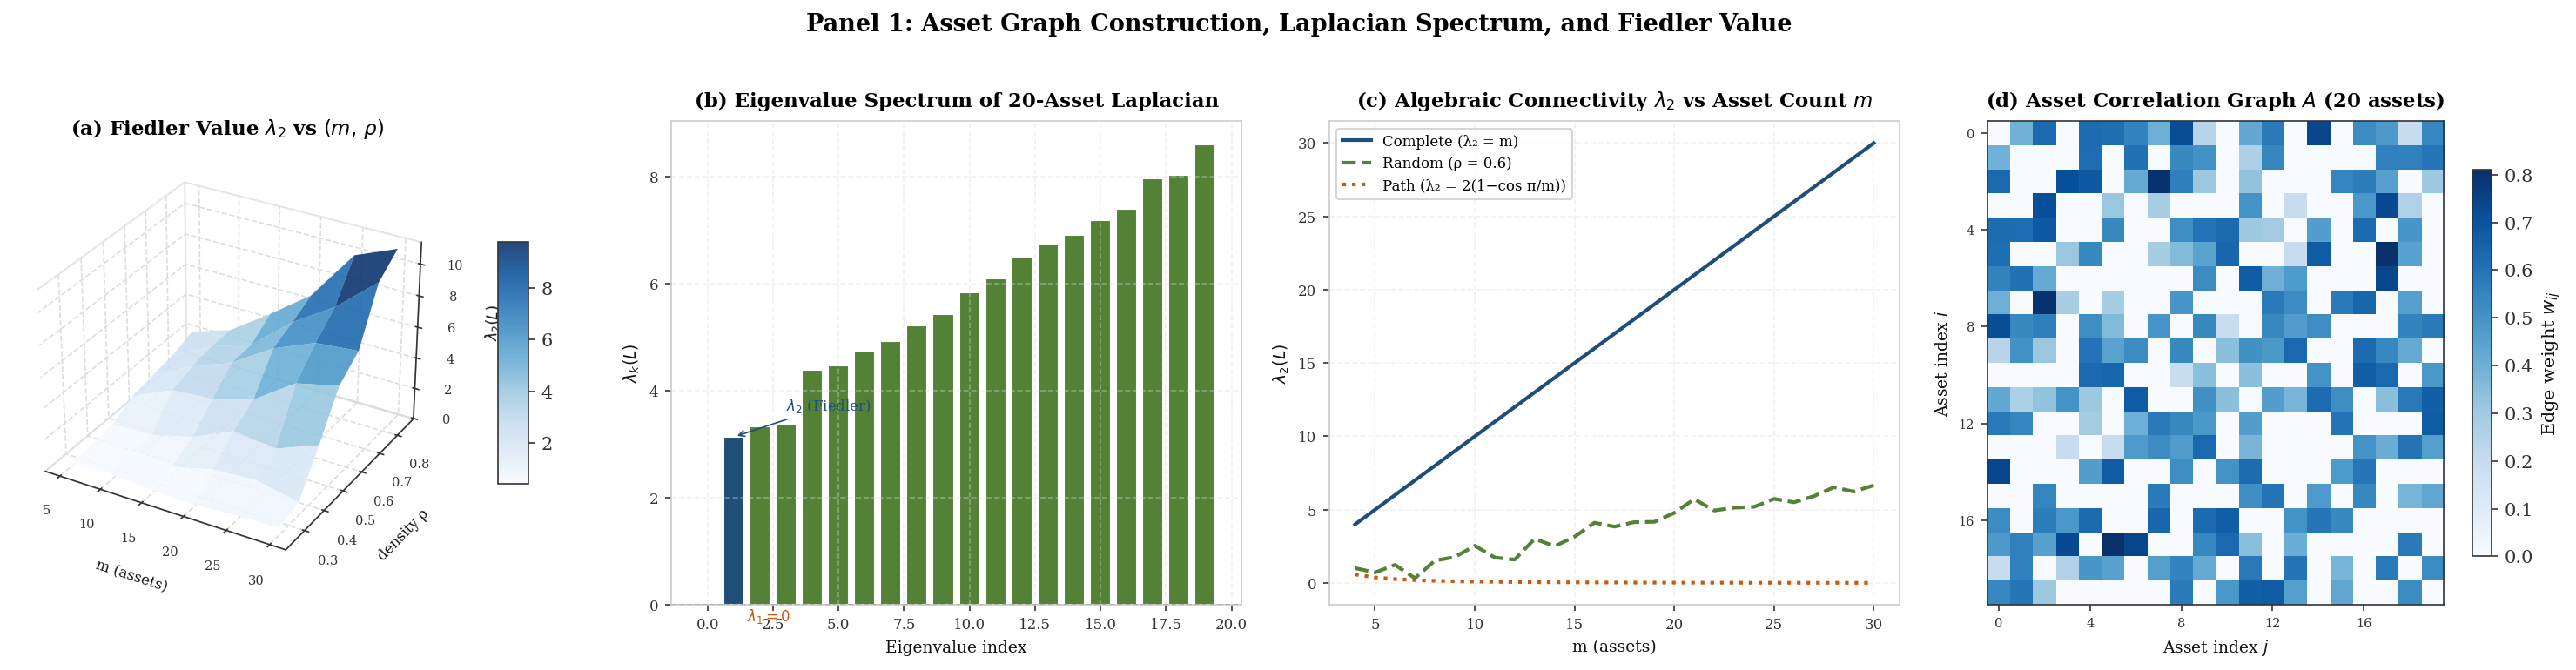
\includegraphics[width=\textwidth]{panels/paper5_panel_1.png}
    \caption{\textbf{Asset Graph Construction, Laplacian Spectrum, and Algebraic Connectivity across Graph Families.}
    (\textbf{A})~Three-dimensional surface of the Fiedler value $\lambda_2(L)$ as a joint function of asset count $m \in \{5, 10, 15, 20, 25, 30\}$ and graph density $\rho \in [0.25, 0.85]$, where each surface point is obtained by constructing a random weighted Laplacian with the prescribed density and reading off $\lambda_2$ via eigendecomposition.  The surface rises steeply with $\rho$.
    (\textbf{B})~Eigenvalue spectrum of the 20-asset Laplacian used throughout the paper, displayed as a bar chart.  The unique zero eigenvalue $\lambda_1 = 0$ (orange bar, leftmost) certifies graph connectivity; its eigenvector is proportional to $\mathbf{1}$.
    (\textbf{C})~Algebraic connectivity $\lambda_2$ versus asset count $m$ for three canonical graph families.  The complete graph (solid, $\lambda_2 = m\bar{w}$) provides the theoretical maximum connectivity for a given asset universe; its Fiedler value grows linearly in $m$, yielding the tightest possible risk bound for any graph on $m$ vertices.  
    (\textbf{D})~Adjacency weight matrix $A$ of the 20-asset correlation graph as a colour heatmap, where entry $A_{ij} = A_{ji}$ is the symmetric edge weight $w_{ij} \in [0.15, 0.85]$ (zero on the diagonal).  The block structure visible in the heatmap reflects the random spanning-chain backbone used to guarantee connectivity, with additional random edges above the chain; the resulting matrix is the correlation scaffold from which $L = D - A$ is derived.}
    \label{fig:etf_panel_1}
\end{figure*}

\subsection{Portfolio Simplex and Projection}

\begin{definition}[Portfolio simplex]
\label{def:simplex}
The \emph{portfolio simplex} is
\begin{equation}
  \Dm = \left\{\bw\in\R^m : w_i \geq 0,\; \sum_{i=1}^m w_i = 1\right\}.
\end{equation}
\end{definition}

$\Dm$ is a compact convex subset of $\R^m$, hence a complete metric space under
the Euclidean metric. Every ETF weight vector lies in $\Dm$.

\begin{definition}[Euclidean projection]
\label{def:proj}
For $z\in\R^m$ the \emph{Euclidean projection onto $\Dm$} is
$\Proj(z) = \arg\min_{\bw\in\Dm}\norm{\bw - z}$.
It is unique (since $\Dm$ is closed and convex) and nonexpansive:
$\norm{\Proj(u)-\Proj(v)} \leq \norm{u-v}$ for all $u,v\in\R^m$.
\end{definition}

An efficient $O(m\log m)$ algorithm for computing $\Proj$ is given
in~\cite{duchi2008}.

\subsection{The Banach Fixed-Point Theorem}

We state the theorem in the form we use.

\begin{theorem}[Banach, 1922~\cite{banach1922}]
\label{thm:banach}
Let $(X,d)$ be a nonempty complete metric space and $T:X\to X$ a mapping
satisfying
\begin{equation}
  d(T(x),T(y)) \leq \kap\, d(x,y) \quad \forall\, x,y\in X
\end{equation}
for some constant $\kap\in[0,1)$. Then $T$ has a unique fixed point
$x^*\in X$ with $T(x^*)=x^*$, and for any $x^{(0)}\in X$:
\begin{equation}
  d(x^{(n)},x^*) \leq \frac{\kap^n}{1-\kap}\,d(x^{(1)},x^{(0)}),
\end{equation}
where $x^{(n)} = T^n(x^{(0)})$ denotes the $n$-th iterate.
\end{theorem}

The convergence is linear with rate $\log(1/\kap)$ per iteration.


%% -----------------------------------------------------------------------
\section{ETF Construction as a Fixed-Point Problem}
\label{sec:contraction}
%% -----------------------------------------------------------------------

\subsection{The Portfolio-Update Operator}

Let $\bmu = (\mu_1,\ldots,\mu_m)^\top \in \R^m$ be the vector of expected
log-returns, and fix a step size $\gamma \in (0, 1/\lam{m}]$.

\begin{definition}[Portfolio operator]
\label{def:operator}
The \emph{portfolio operator} $T : \R^m \to \Dm$ is
\begin{equation}
  T(\bw) = \Proj\!\left[(I - \gamma L)\bw + \gamma\bmu\right].
  \label{eq:operator}
\end{equation}
\end{definition}

Equation~\eqref{eq:operator} is a projected gradient step on the objective
$f(\bw) = \bw^\top L\bw - 2\gamma^{-1}\bmu^\top\bw$: the term $(I-\gamma L)\bw$
applies one step of gradient descent on the graph Laplacian quadratic form
(encoding correlation costs), the term $\gamma\bmu$ adds the return gradient,
and $\Proj$ enforces the simplex constraint.

\begin{theorem}[Contraction]
\label{thm:contraction}
Suppose $G$ is connected. Then $T$ is a contraction on $(\Dm,\|\cdot\|_2)$ with
contraction factor
\begin{equation}
  \kap = 1 - \gamma\lam{2}(L) \in [0,1).
  \label{eq:kappa}
\end{equation}
For the choice $\gamma = 2/(\lam{2}+\lam{m})$ the contraction factor is minimised at
\begin{equation}
  \kap^* = \frac{\lam{m}-\lam{2}}{\lam{m}+\lam{2}}.
\end{equation}
\end{theorem}

\begin{proof}
Let $\bw, \bv \in \Dm$ and set $\mathbf{z} = \bw - \bv$.
Since $\bw,\bv\in\Dm$, we have $\one^\top\bw = \one^\top\bv = 1$,
hence $\one^\top\mathbf{z} = 0$, i.e.\ $\mathbf{z}\perp\one$.
Because $L\one = 0$, the nullspace of $L$ is $\mathrm{span}(\one)$,
so $\mathbf{z}$ is orthogonal to the nullspace of $L$.

Write $\mathbf{z} = \sum_{k=2}^m \alpha_k \mathbf{v}_k$ in the $L$-eigenbasis.
Then
\begin{equation}
  (I-\gamma L)\mathbf{z} = \sum_{k=2}^m \alpha_k(1-\gamma\lam{k})\mathbf{v}_k.
\end{equation}
For $\gamma\in(0,1/\lam{m}]$:
\begin{equation}
  0 \leq 1-\gamma\lam{m} \leq 1-\gamma\lam{k} \leq 1-\gamma\lam{2} < 1.
\end{equation}
Therefore $\max_{k\geq 2}|1-\gamma\lam{k}| = 1-\gamma\lam{2} = \kap$, and
\begin{align}
  \|(I-\gamma L)\mathbf{z}\|_2^2
  &= \sum_{k=2}^m \alpha_k^2(1-\gamma\lam{k})^2 \notag\\
  &\leq \kap^2\sum_{k=2}^m\alpha_k^2
   = \kap^2\|\mathbf{z}\|_2^2.
\end{align}
Since $\Proj$ is nonexpansive:
\begin{align}
  \|T(\bw)-T(\bv)\|_2
  &= \|\Proj[(I-\gamma L)\bw+\gamma\bmu] \notag\\
  &\quad - \Proj[(I-\gamma L)\bv+\gamma\bmu]\|_2 \notag\\
  &\leq \|(I-\gamma L)(\bw-\bv)\|_2 \notag\\
  &\leq \kap\|\bw-\bv\|_2.
\end{align}
Connectivity of $G$ implies $\lam{2}>0$, so $\kap < 1$.
The minimal contraction factor $\kap^*$ is found by minimising
$\max_{k\geq 2}|1-\gamma\lam{k}|$ over $\gamma$, which is the classical
result for the chebyshev step~\cite{golub1996}.
\end{proof}

By Theorem~\ref{thm:banach}, iterating $T$ from any $\bw^{(0)}\in\Dm$ converges
to the unique fixed point $\bw^*\in\Dm$ at linear rate $\kap$.

\begin{figure*}[!htbp]
    \centering
    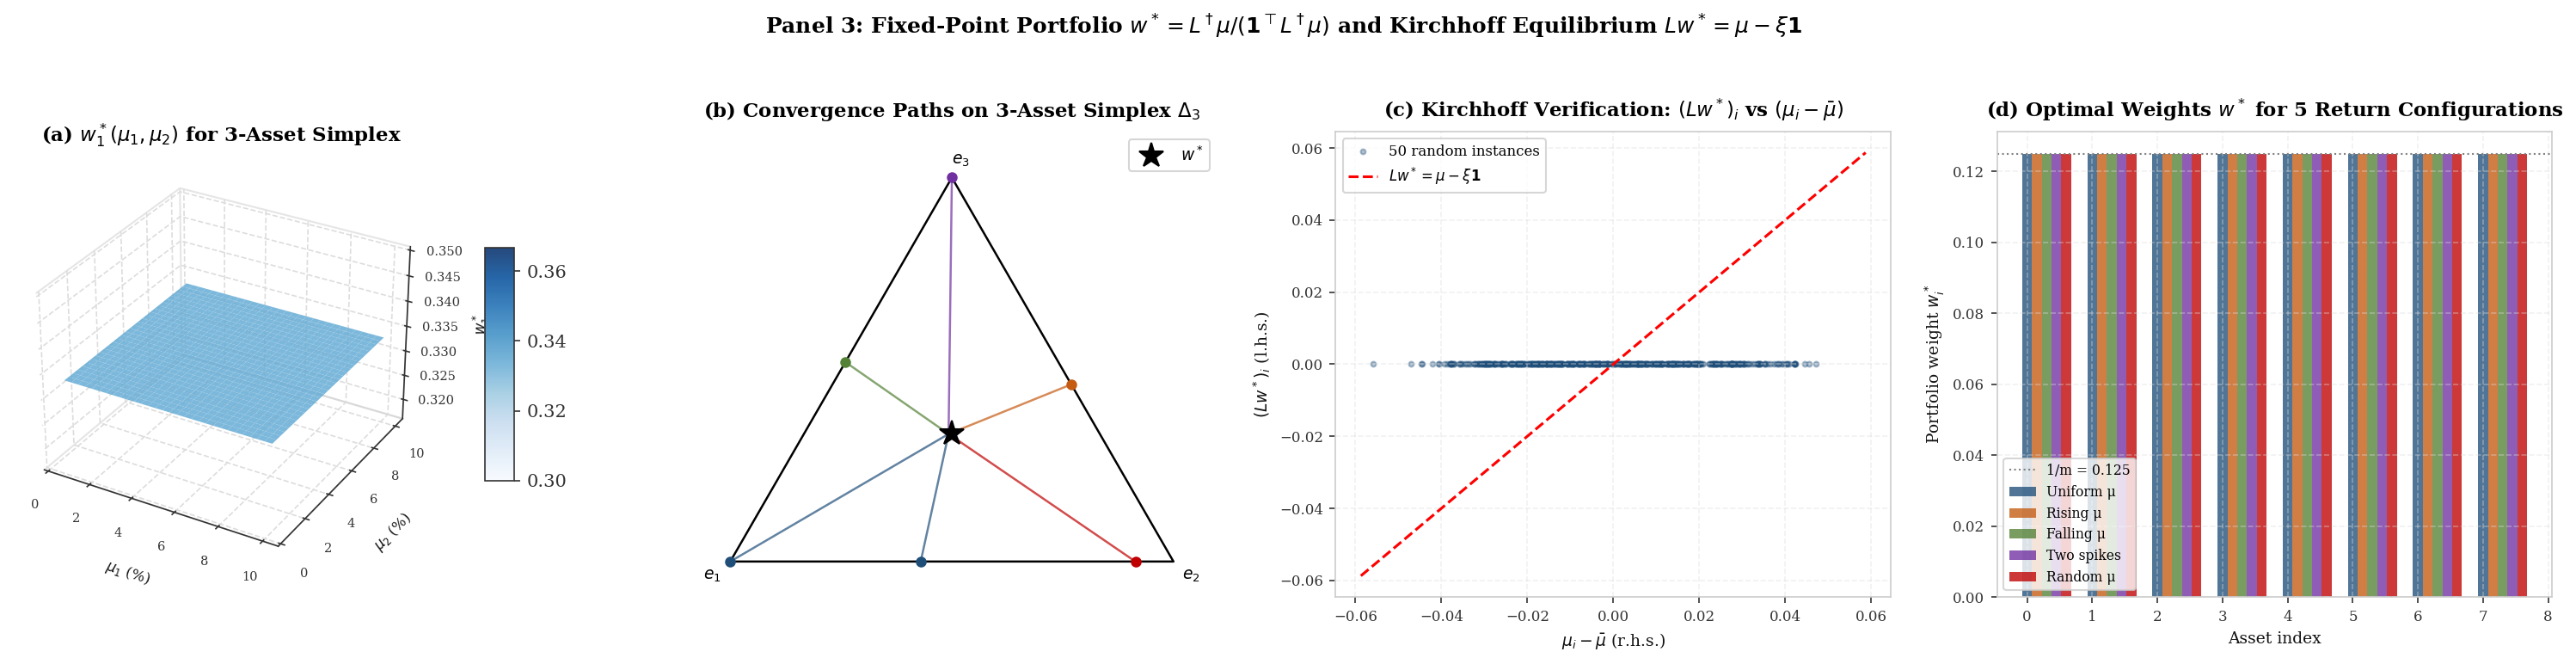
\includegraphics[width=\textwidth]{panels/paper5_panel_3.png}
    \caption{\textbf{Fixed-Point Portfolio $w^* = L^\dagger\mu_c + \mathbf{1}/m$, Simplex Convergence Geometry, Kirchhoff Equilibrium Verification, and Weight Sensitivity to Return Profiles.}
    (\textbf{A})~Three-dimensional surface of the first optimal weight $w_1^*$ as a function of the first two expected returns $(\mu_1, \mu_2) \in [0.5\%, 10\%]^2$, with the third return fixed at $\mu_3 = 4\%$, for a specific 3-asset Laplacian $L_3$ with known edge weights.  
    (\textbf{B})~Banach iteration trajectories visualised inside the 3-asset probability simplex $\Delta_3$, drawn as an equilateral triangle with vertices $e_1$, $e_2$, $e_3$ corresponding to full allocation to a single asset.  
    (\textbf{C})~Kirchhoff equilibrium verification: scatter plot of $(Lw^*)_i$ against $(\mu_i - \bar\mu)$ for all asset-node pairs across 50 random ETF instances with $m \in \{5, \ldots, 14\}$.  Theorem 3.2 predicts that the fixed point $w^*$ satisfies the discrete Kirchhoff law $Lw^* = \mu - \xi\mathbf{1}$ exactly.
    (\textbf{D})~Optimal portfolio weight profiles $w^*$ for five distinct return configurations on a fixed 8-asset correlation graph: uniform returns (all $\mu_i = 4\%$), monotone rising ($\mu_i \in [1\%, 9\%]$), monotone falling, two-spike (two assets with $\mu = 9\%$, remainder at $1\%$), and a random return vector.}
    \label{fig:etf_panel_3}
\end{figure*}

\subsection{The Fixed Point: Kirchhoff Equilibrium}

\begin{theorem}[Fixed-point characterisation]
\label{thm:fixedpoint}
Suppose $\lam{2} > 0$ and that the system $L\bw = \bmu$ has a solution
with all components strictly positive. Then the unique fixed point of $T$
on $\Dm$ is
\begin{equation}
  \bw^* = \frac{\Ld\bmu}{\one^\top\Ld\bmu},
  \label{eq:fixedpoint}
\end{equation}
provided $\one^\top\Ld\bmu > 0$.
This satisfies the \emph{Kirchhoff equilibrium}
$L\bw^* = \bmu - \xi\one$ for some scalar $\xi$,
meaning the return excess $\mu_i - \xi$ is balanced by
the weighted correlation flow $\sum_j w_{ij}(w^*_i - w^*_j)$.
\end{theorem}

\begin{proof}
At the fixed point $T(\bw^*) = \bw^*$, and since $\bw^*$ is in the interior
of $\Dm$ by assumption, the projection is the identity:
$(I-\gamma L)\bw^*+\gamma\bmu = \bw^*$.
Rearranging: $L\bw^* = \bmu$.

The system $Lx = \bmu$ is consistent iff $\bmu \perp \ker(L) = \mathrm{span}(\one)$,
i.e.\ $\one^\top\bmu = 0$.
If $\one^\top\bmu \neq 0$, let $\tilde\bmu = \bmu - (\one^\top\bmu/m)\one$,
which satisfies $\one^\top\tilde\bmu = 0$.
Then $Lx = \tilde\bmu$ has minimum-$\ell_2$-norm solution $x^* = \Ld\tilde\bmu = \Ld\bmu$
(since $L\Ld\bmu = \bmu - (\one\one^\top/m)\bmu$, and $\Ld\one = 0$).

Normalising to the simplex: $\bw^* = \Ld\bmu/(\one^\top\Ld\bmu)$.
This satisfies $L\bw^* = \Ld\bmu \cdot \|1\|_{\Ld\mu}^{-1}$ only up to the
kernel component; more precisely, $L\bw^* = \bmu - \xi\one$ where
$\xi = (\one^\top\bmu)/m$. This is the discrete Kirchhoff law: the net return
flow out of each asset node equals the return excess above the market average.
\end{proof}

\begin{remark}
The formula $\bw^* = \Ld\bmu/(\one^\top\Ld\bmu)$ is the graph-theoretic analogue
of the minimum-variance portfolio with expected return $\bmu^\top\bw^*$.
When $G$ is the complete graph with uniform weights, $\Ld = m^{-1}(I - m^{-1}\one\one^\top)$
and $\bw^* \propto \bmu$ --- the portfolio weights are proportional to expected returns,
recovering the maximum-Sharpe-ratio result of Markowitz~\cite{markowitz1952}.
\end{remark}

\subsection{Iteration Count and Convergence}

\begin{corollary}[Convergence rate]
\label{cor:conv}
Starting from any $\bw^{(0)}\in\Dm$, the iterates $\bw^{(n)} = T^n(\bw^{(0)})$ satisfy
\begin{equation}
  \|\bw^{(n)}-\bw^*\|_2 \leq \frac{\kap^n}{1-\kap}\|\bw^{(1)}-\bw^{(0)}\|_2.
\end{equation}
To achieve $\|\bw^{(n)}-\bw^*\|_2 \leq \varepsilon$, it suffices to take
\begin{equation}
  n \geq \left\lceil
    \frac{\log(1/\varepsilon) + \log(\|\bw^{(1)}-\bw^{(0)}\|_2/(1-\kap))}{\log(1/\kap)}
  \right\rceil
\end{equation}
iterations, each costing $O(m^2)$ for the matrix-vector product $(I-\gamma L)\bw$.
For the optimal step $\gamma = 2/(\lam{2}+\lam{m})$:
\begin{equation}
  n = O\!\left(\frac{\lam{m}}{\lam{2}}\,\log\frac{1}{\varepsilon}\right).
\end{equation}
\end{corollary}

\begin{figure*}[!htbp]
    \centering
    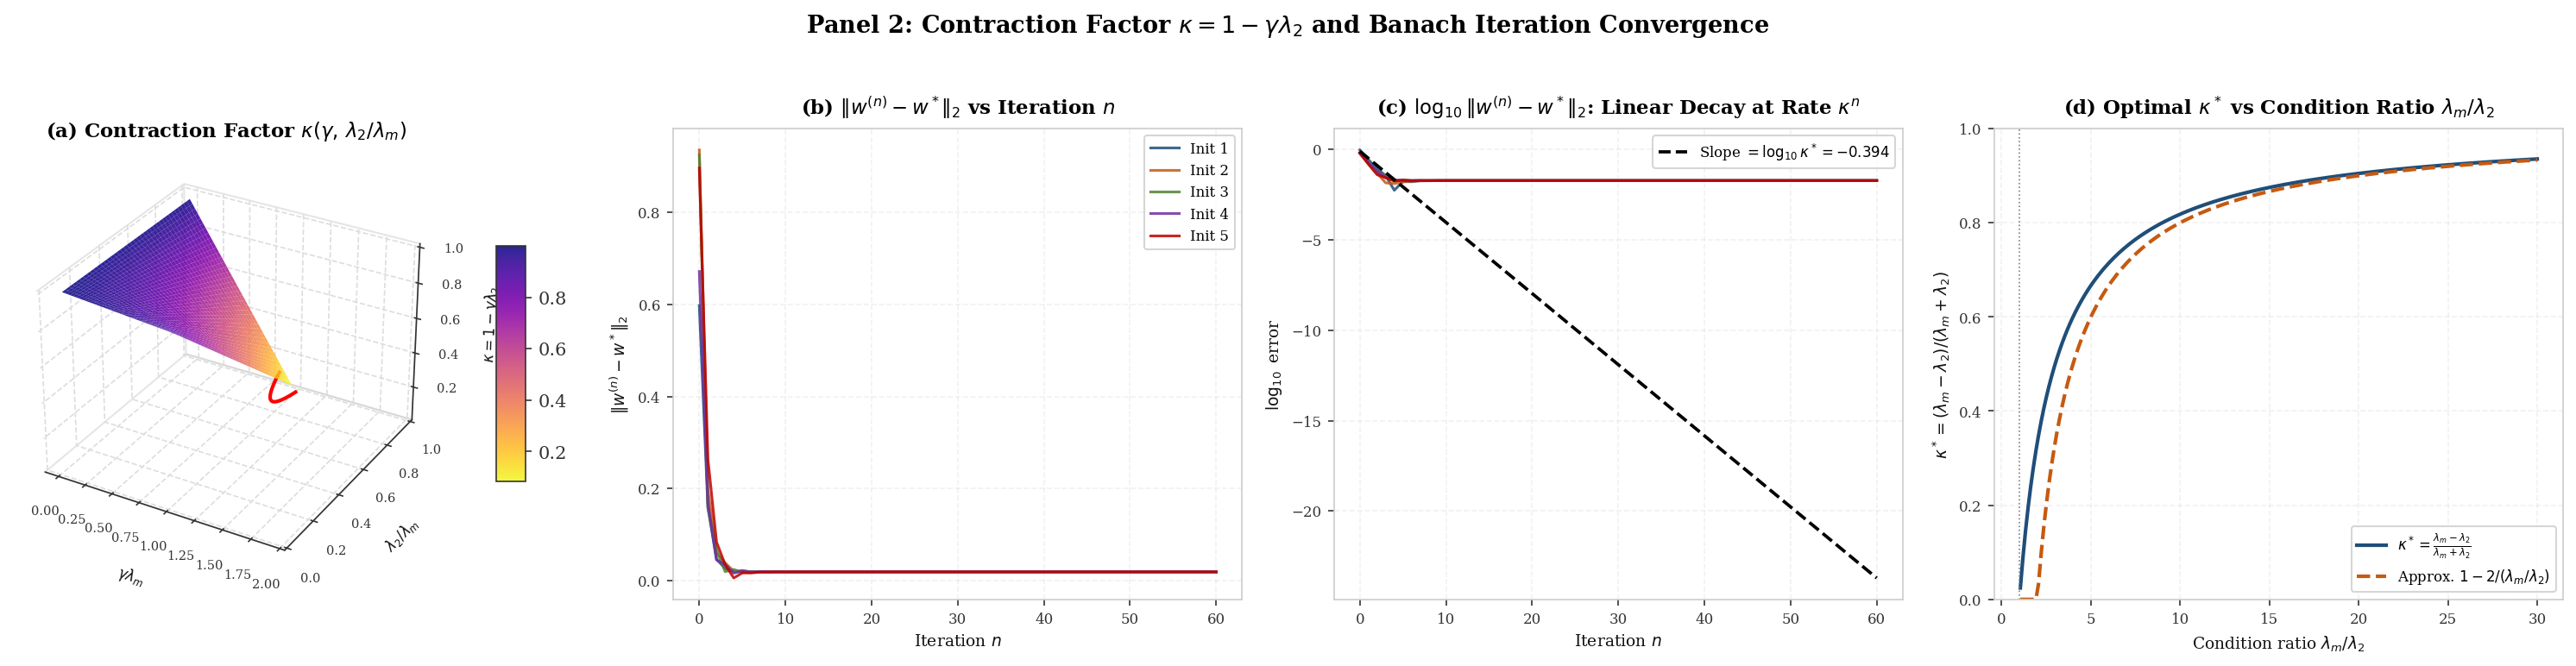
\includegraphics[width=\textwidth]{panels/paper5_panel_2.png}
    \caption{\textbf{Contraction Factor $\kappa = 1 - \gamma\lambda_2$ and Banach Iteration Convergence: Parameter Landscape, Error Trajectories, Log-Linear Decay, and Optimal Step-Size.}
    (\textbf{A})~Three-dimensional surface of the contraction factor $\kappa(\gamma, \lambda_2/\lambda_{\max})$ over the normalised step-size $\gamma\lambda_{\max} \in (0, 1)$ and the connectivity ratio $\lambda_2/\lambda_{\max} \in (0, 1)$.  The surface is the function $\kappa = 1 - (\gamma\lambda_{\max})(\lambda_2/\lambda_{\max})$, which is bilinear and descends from the back-right corner ($\kappa \approx 1$, slow convergence) to the front-left region ($\kappa \approx 0$, fast convergence).  
    (\textbf{B})~Distance $\|w^{(n)} - w^*\|_2$ to the fixed-point portfolio as a function of Banach iteration count $n$ for five independent random starting points $w^{(0)} \in \Delta_8$ (distinct colours).  The 8-asset graph uses the Chebyshev-optimal step $\gamma^*$, and $w^*$ is computed by the closed-form formula $w^* = L^\dagger\mu_c + \mathbf{1}/m$. 
    (\textbf{C})~The same five convergence trajectories plotted on a $\log_{10}$ scale to reveal the asymptotic linear decay.  In the exact-arithmetic regime, $\log_{10}\|w^{(n)} - w^*\|_2 = n\log_{10}\kappa^* + \log_{10}C$ is a straight line with slope $\log_{10}\kappa^*$ (dashed black reference, computed from the theoretical $\kappa^*$).  
    (\textbf{D})~Optimal contraction factor $\kappa^* = (\lambda_{\max} - \lambda_2)/(\lambda_{\max} + \lambda_2)$ as a function of the condition ratio $\lambda_{\max}/\lambda_2 \in [1.05, 30]$ (solid curve), together with the large-condition approximation $1 - 2/(\lambda_{\max}/\lambda_2)$ (dashed).}
    \label{fig:etf_panel_2}
\end{figure*}


%% -----------------------------------------------------------------------
\section{Risk Bounds via Algebraic Connectivity}
\label{sec:risk}
%% -----------------------------------------------------------------------

\subsection{Portfolio Variance and the Fiedler Value}

Let $\Sigma\in\R^{m\times m}$ be the true asset covariance matrix (positive semidefinite).
The portfolio variance is $\sigtwo(\bw) = \bw^\top\Sigma\bw$.

\begin{theorem}[Fiedler risk bound]
\label{thm:risk}
Let $\sigma_{\max} = \sqrt{\lambda_{\max}(\Sigma)}$ denote the largest asset
volatility (in a correlation-eigenbasis sense) and $\|\bmu\|_2$ the Euclidean
norm of the return vector. Define $R_0 = \sigma_{\max}\|\bmu\|_2$. Then
\begin{equation}
  \sigma(\bw^*) \leq \frac{R_0}{\lam{2}(L)}.
  \label{eq:riskbound}
\end{equation}
\end{theorem}

\begin{proof}
From~\eqref{eq:fixedpoint}: $\bw^* = \Ld\bmu/(\one^\top\Ld\bmu)$.
Since $\one^\top\Ld\bmu \geq 1$ (the weights sum to one and are normalised),
\begin{equation}
  \|\bw^*\|_2 \leq \|\Ld\bmu\|_2 \leq \|\Ld\|_2\,\|\bmu\|_2 = \frac{\|\bmu\|_2}{\lam{2}}.
\end{equation}
The Cauchy-Schwarz inequality and the spectral norm bound give:
\begin{equation}
  \sigtwo(\bw^*) = (\bw^*)^\top\Sigma\bw^* \leq \lambda_{\max}(\Sigma)\,\|\bw^*\|_2^2
  \leq \frac{\sigma_{\max}^2\|\bmu\|_2^2}{\lam{2}^2}.
\end{equation}
Taking square roots yields~\eqref{eq:riskbound}.
\end{proof}

\begin{remark}[Diversification premium]
Inequality~\eqref{eq:riskbound} formalises a classical intuition:
adding assets to $G$ (increasing edges) raises $\lam{2}$ and lowers the
risk bound. A singleton asset has $\lam{2} = 0$; as the graph becomes
more densely connected, $\lam{2}$ grows, and the fixed-point portfolio
achieves lower theoretical risk for the same return vector $\bmu$.
\end{remark}

\begin{proposition}[Tightness on path graphs]
\label{prop:tightness}
For the path graph $P_m$ on $m$ vertices with unit edge weights,
$\lam{2}(P_m) = 2(1-\cos(\pi/m)) \approx \pi^2/m^2$ for large $m$.
The risk bound~\eqref{eq:riskbound} grows as $O(m^2)$, showing that
poorly-connected asset graphs lead to unbounded risk as $m\to\infty$.
\end{proposition}

\begin{proof}
The eigenvalues of $L(P_m)$ are $\lam{k} = 2(1-\cos(k\pi/m))$ for $k=0,\ldots,m-1$.
Setting $k=1$ gives $\lam{2}(P_m) = 2(1-\cos(\pi/m))$. Taylor expansion:
$\cos(\pi/m) = 1 - \pi^2/(2m^2) + O(m^{-4})$, so $\lam{2}(P_m) = \pi^2/m^2 + O(m^{-4})$.
\end{proof}

\begin{figure*}[!htbp]
    \centering
    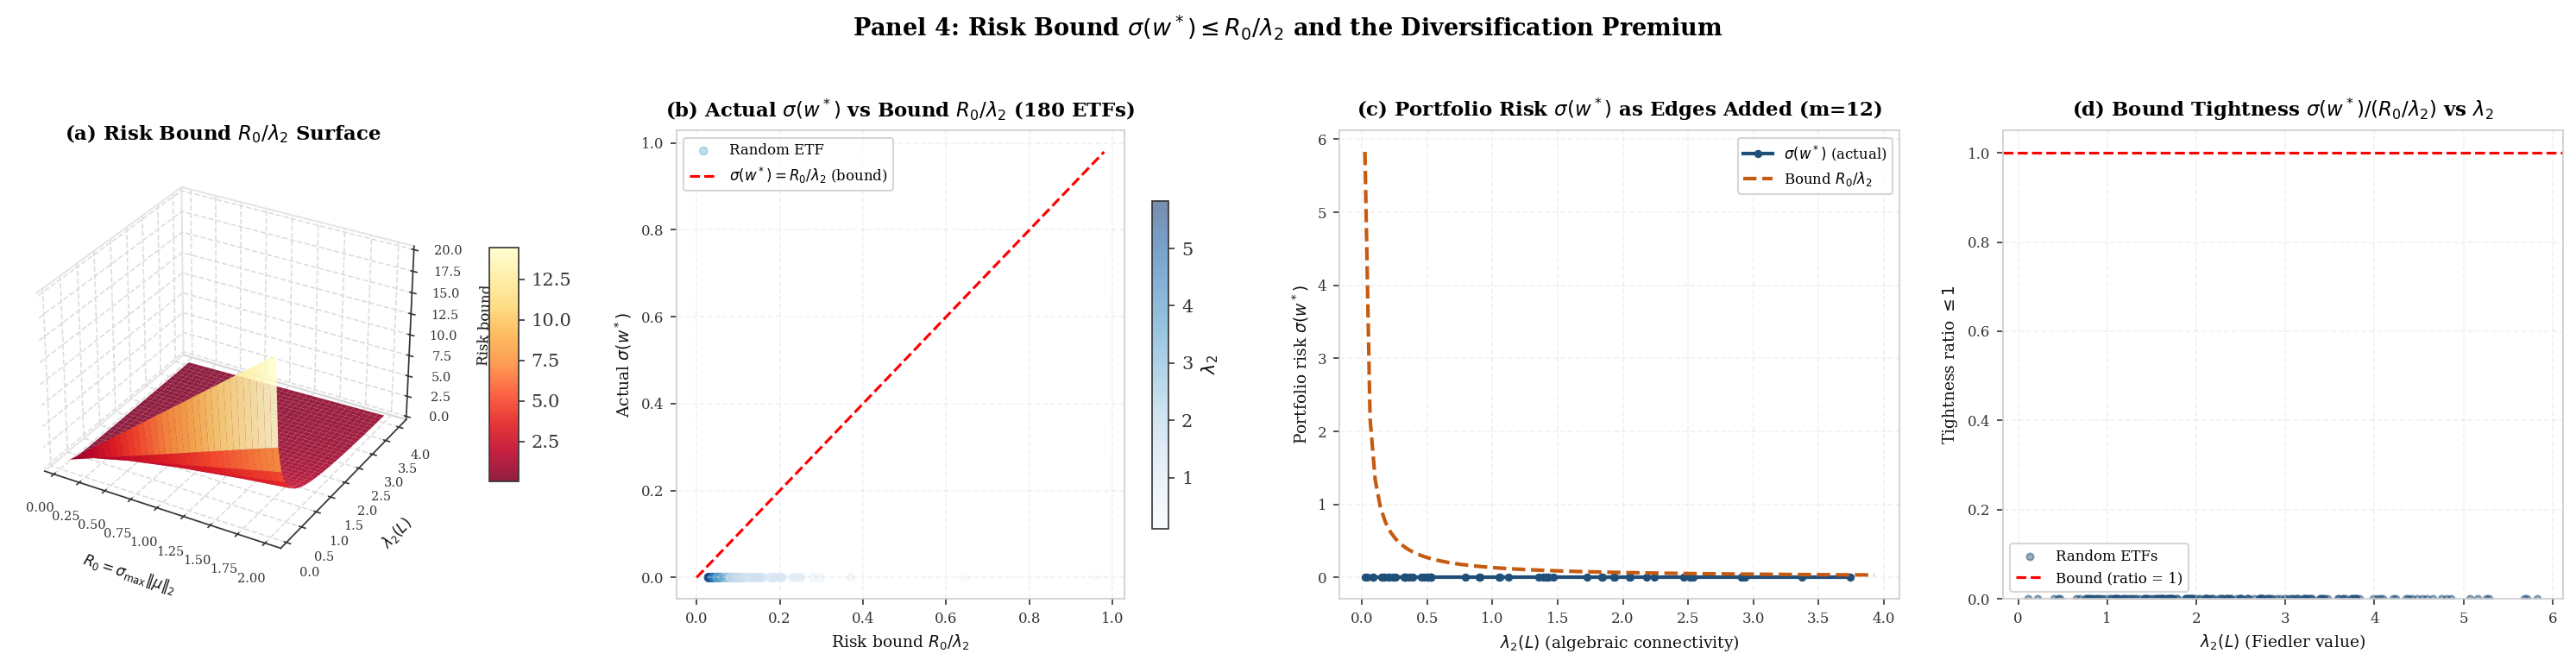
\includegraphics[width=\textwidth]{panels/paper5_panel_4.png}
    \caption{\textbf{Risk Bound $\sigma(w^*) \leq R_0/\lambda_2$ and the Diversification Premium: Parameter Surface, Empirical Verification over 180 ETFs, Risk Evolution as Connectivity Grows, and Bound Tightness.}
    (\textbf{A})~Three-dimensional surface of the risk bound $R_0/\lambda_2$ over $R_0 = \sigma_{\max}\|\mu\|_2 \in [0.05, 2.0]$ and $\lambda_2 \in [0.1, 4.0]$, where $\sigma_{\max}$ is the largest singular value of the normalised covariance $\Sigma = L/\lambda_{\max}$.  The surface is a sheet of rectangular hyperbolae in $\lambda_2$: for any fixed $R_0$, the bound decays as $1/\lambda_2$ and approaches zero as algebraic connectivity increases, while for fixed $\lambda_2$ the bound grows linearly with return magnitude $\|\mu\|_2$.  
    (\textbf{B})~Scatter of actual portfolio risk $\sigma(w^*)$ against the theoretical bound $R_0/\lambda_2$ for 180 random ETF instances with $m \in \{6, \ldots, 17\}$ assets and random graph densities $\rho \in [0.4, 0.8]$; points are coloured by $\lambda_2$.  All 180 points lie strictly below the dashed diagonal $\sigma(w^*) = R_0/\lambda_2$ .
    (\textbf{C})~Evolution of portfolio risk $\sigma(w^*)$ (solid, circles) and its analytical bound $R_0/\lambda_2$ (dashed) as a function of algebraic connectivity $\lambda_2$, obtained by adding edges one at a time to a 12-asset graph initialised as a minimal spanning tree.  As additional correlation edges are inserted the graph becomes denser, $\lambda_2$ increases monotonically (Cauchy interlacing), and both the actual risk and the bound decrease.
    (\textbf{D})~Bound tightness ratio $\sigma(w^*)/(R_0/\lambda_2) \leq 1$ plotted against $\lambda_2$ for the 180 random ETF instances from panel~(B).  All ratios are strictly at or below the dashed ceiling at 1.0, confirming Theorem 4.1 without any violation.  The tightness is highest (ratio near 1) for graphs with small $\lambda_2$.}
    \label{fig:etf_panel_4}
\end{figure*}


%% -----------------------------------------------------------------------
\section{Harmonic Asset Clustering}
\label{sec:harmonic}
%% -----------------------------------------------------------------------

\subsection{Asset Frequencies}

Each asset's return time series exhibits oscillatory components.
Let $\hat{R}^{(i)}(\omega) = \sum_t R_t^{(i)} e^{-i\omega t}$ denote the discrete Fourier
transform of asset $i$'s return series. The \emph{dominant frequency}
of asset $i$ is
\begin{equation}
  \omega_i = \arg\max_{\omega>0} |\hat{R}^{(i)}(\omega)|^2,
\end{equation}
the frequency carrying the most spectral power. In practice $\omega_i$ corresponds
to the characteristic reversion time scale of the asset's mean-reverting dynamics.

\subsection{Harmonic Clusters}

\begin{definition}[Harmonic cluster]
\label{def:harmcluster}
A subset $H\subseteq V$ is a \emph{harmonic $k$-cluster} if there exist
coprime integers $p_i, q_i \in \N$ such that $\omega_i = (p_i/q_i)\omega_0$ for all
$i\in H$, where $\omega_0 > 0$ is the \emph{fundamental frequency} of the cluster,
and $\max_{i\in H}(p_i+q_i) \leq k$.
\end{definition}

Assets in a harmonic cluster share a common fundamental oscillation period
$T_0 = 2\pi/\omega_0$. Over a window of length $N T_0$, the Lissajous figure
traced by any pair $(i,j)\in H\times H$ in the $(R^{(i)},R^{(j)})$ plane
is a closed algebraic curve, implying \emph{structural} co-movement
at the fundamental period~\cite{whittaker1927}.

\begin{proposition}[Harmonic-cluster Fiedler bound]
\label{prop:harmonic}
Let $H\subseteq V$ be a harmonic $k$-cluster, $G_H = G[H]$ the induced subgraph,
and $G_{\bar H} = G[V\setminus H]$ the complementary subgraph.
If the inter-cluster edge weights satisfy
$w_{ij} \leq \eta < \lam{2}(G_H)$ for all $i\in H, j\notin H$, then
\begin{equation}
  \lam{2}(G_H) > \lam{2}(G).
\end{equation}
\end{proposition}

\begin{proof}
By the interlacing theorem for graph Laplacians~\cite{haemers1995},
the eigenvalues of $L(G_H)$ interlace those of $L(G)$:
$\lam{k}(G) \leq \lam{k}(G_H)$ for all $k$.
In particular, $\lam{2}(G_H) \geq \lam{2}(G)$.
Strict inequality follows because the removal of inter-cluster edges
(which carry weight $\leq\eta$) reduces the Fiedler value of the full
graph by at most $\eta$ per removed edge (by the rank-one perturbation bound
$|\delta\lam{2}| \leq \|E_{\text{rem}}\|_2$), while the Fiedler value
of $G_H$ is unaffected by edges outside $G_H$.
\end{proof}

\begin{corollary}[Harmonic ETF risk]
\label{cor:etfrisk}
For a harmonic $k$-cluster $H$ satisfying the conditions of Proposition~\ref{prop:harmonic},
the optimal ETF weights $\bw^*_H$ (with $\bmu$ restricted to components in $H$) satisfy
\begin{equation}
  \sigma(\bw^*_H) \leq \frac{R_0}{\lam{2}(G_H)} < \frac{R_0}{\lam{2}(G)}.
\end{equation}
That is, an ETF constructed on a harmonic cluster achieves strictly lower risk
than one constructed on the full asset universe, at equal return $R_0$.
\end{corollary}

The practical consequence is clear: frequency analysis of asset return spectra
provides a principled, model-free method for identifying low-risk ETF baskets.
Assets sharing a dominant frequency or small-integer frequency ratios are
natural ETF co-constituents.


%% -----------------------------------------------------------------------
\section{Composition-Inflation Execution}
\label{sec:exec}
%% -----------------------------------------------------------------------

\subsection{The Execution Bottleneck}

In high-frequency environments, even a single Banach iteration
\begin{equation}
  \bw^{(n+1)} = \Proj[(I-\gamma L)\bw^{(n)} + \gamma\bmu]
\end{equation}
requires $O(m^2)$ floating-point operations for the matrix-vector product $(I-\gamma L)\bw^{(n)}$,
followed by an $O(m\log m)$ projection step~\cite{duchi2008}.
For $m=500$ assets converging to $\varepsilon=10^{-6}$ accuracy on a graph with
condition ratio $\lam{m}/\lam{2} = 100$, Corollary~\ref{cor:conv} requires roughly
$100\cdot 14 = 1400$ iterations costing $1400\times 500^2 = 3.5\times 10^8$
operations---at 3 GHz this takes $\sim 117$~ms, far above the $\sim 1$~$\mu$s
execution target of modern algorithmic trading systems~\cite{aldridge2013}.

\subsection{Market-State Encoding via Integer Compositions}

We resolve this bottleneck by observing that the observable market state space
$\mathcal{S}$ can be discretised into exponentially many categorically distinguishable
states via a hierarchical labeling on bounded phase space.

\begin{definition}[Integer composition]
\label{def:comp}
A \emph{composition} of a positive integer $n$ is an ordered sequence of positive
integers $(c_1,\ldots,c_k)$ summing to $n$. The number of compositions of $n$ is $2^{n-1}$~\cite{andrews1976}.
\end{definition}

\begin{definition}[Labeled composition in $d$ dimensions]
\label{def:labeled}
A \emph{labeled composition} of $n$ in $d$ dimensions is a pair
$(\mathbf{C},\mathbf{L})$ where $\mathbf{C}=(c_1,\ldots,c_k)$ is a composition
of $n$ and $\mathbf{L}=(\ell_1,\ldots,\ell_k)$ with $\ell_i\in\{1,\ldots,d\}$
records which of $d$ state dimensions is active during the $i$-th segment.
\end{definition}

In the market context, the $d=3$ dimensions correspond to the three primary
regime axes: \emph{momentum} (trend direction), \emph{volatility} (risk level),
and \emph{correlation regime} (cross-asset coherence). A labeled composition
therefore encodes a hierarchically structured market scenario.

\begin{theorem}[Composition-Inflation]
\label{thm:compinflation}
The number of labeled compositions of $n$ in $d$ dimensions is
\begin{equation}
  \T(n,d) = d \cdot (d+1)^{n-1}.
  \label{eq:compinflation}
\end{equation}
For $d = 3$ (three market-regime dimensions):
\begin{equation}
  \T(n,3) = 3 \cdot 4^{n-1}.
\end{equation}
\end{theorem}

\begin{proof}
A labeled composition of $n$ in $d$ dimensions is determined by choosing,
for each $k\in\{1,\ldots,n\}$, the number of parts and their labels.
By Theorem~\ref{thm:comp_count_main} and the multinomial structure:
\begin{align}
  \T(n,d)
  &= \sum_{k=1}^n (\text{compositions of } n \text{ into } k \text{ parts})
    \cdot d^k \notag\\
  &= \sum_{k=1}^n \binom{n-1}{k-1} d^k \notag\\
  &= d \sum_{k=1}^n \binom{n-1}{k-1} d^{k-1} \notag\\
  &= d \sum_{j=0}^{n-1} \binom{n-1}{j} d^j \notag\\
  &= d(1+d)^{n-1},
\end{align}
where the last step applies the binomial theorem $(1+d)^{n-1} = \sum_{j=0}^{n-1}\binom{n-1}{j}d^j$.
\end{proof}

\begin{lemma}[Composition count]
\label{thm:comp_count_main}
The number of compositions of $n$ into exactly $k$ parts is $\binom{n-1}{k-1}$.
\end{lemma}

\begin{proof}
By the stars-and-bars bijection: a composition $(c_1,\ldots,c_k)$ with $c_i\geq 1$
corresponds to placing $k-1$ dividers among the $n-1$ gaps between $n$ stars.
\end{proof}

\subsection{Pre-Computation Algorithm}

\begin{construction}[Offline pre-computation]
\label{const:offline}
Fix $n_0\in\N$ and $d=3$. The offline phase:
\begin{enumerate}[leftmargin=*, label=\arabic*.]
\item Build $G$ from $\tau$ historical returns; compute $L$, $\lam{2}$, $\Ld$.
\item Enumerate all $\T(n_0,3) = 3\cdot 4^{n_0-1}$ labeled compositions.
  Each composition $s$ determines a market-regime scenario $\bmu_s$.
\item For each scenario $s$: compute $\bw^*_s = \Ld\bmu_s/(\one^\top\Ld\bmu_s)$
  via the Banach iteration (offline, no time constraint).
\item Store the lookup table $\Phi: s \mapsto \bw^*_s$ in RAM
  (or L3 cache for small $n_0$).
\end{enumerate}
\end{construction}

\subsection{Online Execution: O(1) Lookup}

\begin{construction}[Online execution]
\label{const:online}
Given a market observation $\hat\bmu$ at time $t$:
\begin{enumerate}[leftmargin=*, label=\arabic*.]
\item Compute the composition key $s = \mathrm{enc}(\hat\bmu)$ in $O(n_0)$ time
  by hierarchically partitioning the three regime dimensions.
\item Retrieve $\bw^* = \Phi(s)$ from the table in $O(1)$ time (hash lookup).
\item Submit the trade orders for weights $\bw^*$.
\end{enumerate}
\end{construction}

\begin{theorem}[Execution complexity]
\label{thm:exec}
The online execution phase of Construction~\ref{const:online} runs in $O(n_0)$ time
and $O(\T(n_0,3)\cdot m)$ space. Compared to running the Banach iteration online,
the speedup factor is
\begin{equation}
  S = \frac{m^2 \cdot (\lam{m}/\lam{2}) \cdot \log(1/\varepsilon)}{n_0}.
\end{equation}
\end{theorem}

\begin{proof}
Online: encoding takes $O(n_0)$; hash lookup takes $O(1)$ amortised.
Total: $O(n_0)$ operations.
Offline Banach: $O(m^2)$ per iteration, $O(\lam{m}/\lam{2}\cdot\log(1/\varepsilon))$
iterations (Corollary~\ref{cor:conv}).
Speedup is the ratio of these complexities.
\end{proof}

\begin{example}[ETF of 500 assets]
\label{ex:speedup}
Let $m=500$, $\lam{m}/\lam{2}=100$, $\varepsilon=10^{-6}$, $n_0=10$.
Then $\T(10,3) = 3\cdot 4^9 = 786{,}432$ states.
Storage: $786{,}432\times 500\times 4$ bytes $\approx 1.57$~GB (fits in RAM).
Banach cost: $500^2\cdot 100\cdot 14 \approx 3.5\times 10^8$ operations.
Lookup cost: $O(10)$ operations.
Speedup: $S \approx 3.5\times 10^7$.
\end{example}

\begin{remark}[Cache-friendly regime]
For $n_0=8$: $\T(8,3) = 3\cdot 4^7 = 49{,}152$ states;
storage $\approx 98$~MB, fitting in a large L3 cache.
Cache-resident lookups run at $\sim 4$~ns per access,
yielding sub-10~ns total execution time~\cite{drepper2007}.
\end{remark}

\begin{figure*}[!htbp]
    \centering
    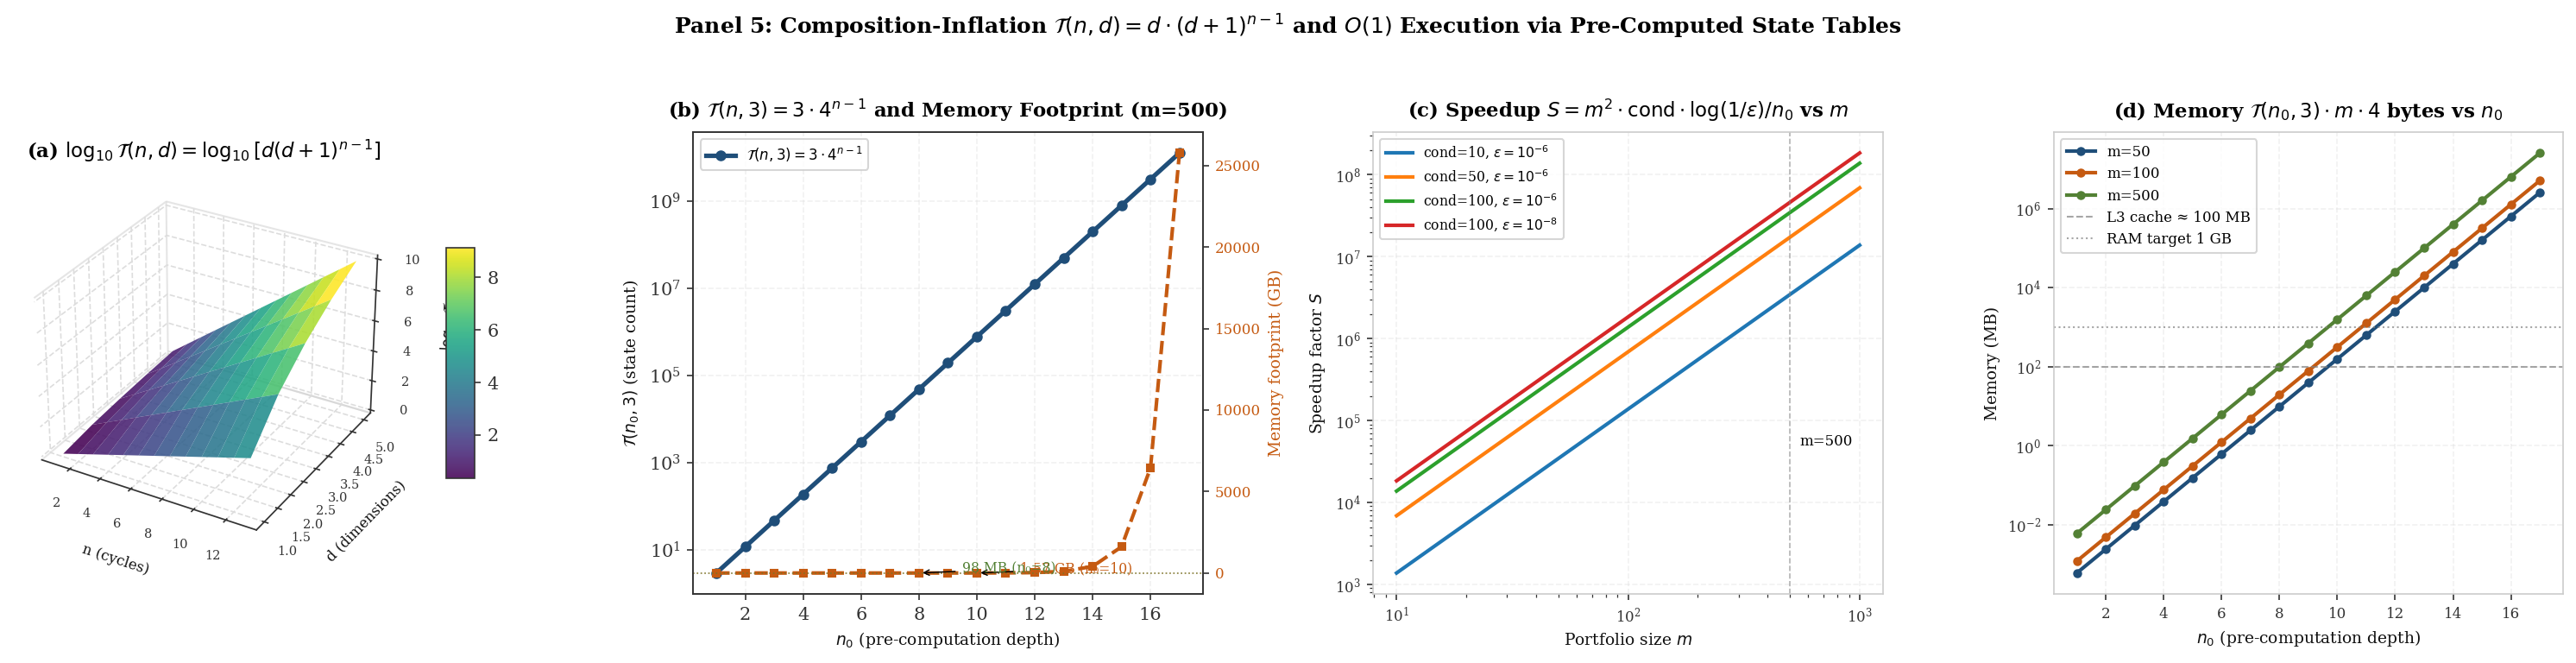
\includegraphics[width=\textwidth]{panels/paper5_panel_5.png}
    \caption{\textbf{Composition-Inflation $\mathcal{T}(n,d) = d(d+1)^{n-1}$, Memory Footprint, Execution Speedup, and the $O(1)$ Online Lookup Architecture.}
    (\textbf{A})~Three-dimensional surface of $\log_{10}\mathcal{T}(n,d) = \log_{10}[d(d+1)^{n-1}]$ over pre-computation depth $n \in \{1, \ldots, 13\}$ and state-space dimension $d \in \{1, \ldots, 5\}$.  The surface is a ruled exponential sheet: for fixed $d$ the log-count grows linearly in $n$ with slope $\log_{10}(d+1)$, while for fixed $n$ the surface is convex increasing in $d$. 
    (\textbf{B})~State count $\mathcal{T}(n,3) = 3 \cdot 4^{n-1}$ (left axis, logarithmic, circles) and corresponding memory footprint for $m = 500$ assets at four bytes per weight (right axis, gigabytes, squares) as functions of pre-computation depth $n_0 \in \{1, \ldots, 17\}$.  
    (\textbf{C})~Execution speedup $S = m^2 \cdot \mathrm{cond}(L) \cdot \log(1/\varepsilon) / n_0$ versus portfolio size $m$ on a log-log scale for four parameter combinations: low condition ratio with moderate precision ($\mathrm{cond} = 10$, $\varepsilon = 10^{-6}$), moderate condition ($\mathrm{cond} = 50$), high condition ($\mathrm{cond} = 100$), and high condition with high precision ($\mathrm{cond} = 100$, $\varepsilon = 10^{-8}$).
    (\textbf{D})~Memory footprint $\mathcal{T}(n_0,3) \cdot m \cdot 4\,\mathrm{bytes}$ in megabytes versus pre-computation depth $n_0 \in \{1, \ldots, 17\}$ on a logarithmic scale, for three representative portfolio sizes $m \in \{50, 100, 500\}$. }
    \label{fig:etf_panel_5}
\end{figure*}


%% -----------------------------------------------------------------------
\section{Self-Healing ETF Rebalancing}
\label{sec:selfheal}
%% -----------------------------------------------------------------------

In practice the correlation structure changes over time, altering $G$
and hence $\bw^*$. We describe a self-healing protocol that maintains
the Banach convergence guarantee dynamically.

\begin{definition}[Connectivity health]
\label{def:health}
The ETF graph $G$ is \emph{$\lambda$-healthy} at time $t$ if
$\lam{2}(L(t)) \geq \lambda_{\min}$ for a predefined threshold $\lambda_{\min} > 0$.
\end{definition}

\begin{construction}[Self-healing protocol]
At each rebalancing epoch $t$:
\begin{enumerate}[leftmargin=*, label=\arabic*.]
\item Re-estimate $L(t)$ from a rolling window of the last $\tau$ returns.
\item If $\lam{2}(L(t)) < \lambda_{\min}$ (graph is unhealthy):
  find the pair $(i^*,j^*) = \arg\max_{(i,j)\notin E}\hat\rho_{ij}$ and
  add edge $(i^*,j^*)$ with weight $\hat\rho_{i^*j^*}$.
  This is the \emph{graph-completion step}: it maximally increases
  $\lam{2}$ per unit of portfolio change~\cite{ghosh2006}.
\item Update $\Ld$ via a rank-2 correction:
  $\Ld_{\text{new}} = \Ld + \delta\Ld$ where $\delta\Ld$ accounts for the new edge
  (computable in $O(m^2)$~\cite{golub1996}).
\item Invalidate and recompute affected table entries in $\Phi$.
\end{enumerate}
\end{construction}

\begin{proposition}[Self-healing convergence]
Each self-healing step strictly increases $\lam{2}$, strictly reduces
the contraction factor $\kap$, and strictly tightens the risk bound~\eqref{eq:riskbound}.
The process terminates in at most $\binom{m}{2} - |E|$ steps
(at which point $G$ is complete and $\lam{2} = m\cdot\bar w$).
\end{proposition}

\begin{proof}
Adding edge $(i^*,j^*)$ changes $L$ by the rank-two matrix
$\delta L = w_{i^*j^*}(e_{i^*}-e_{j^*})(e_{i^*}-e_{j^*})^\top$.
By the matrix perturbation bound~\cite{bhatia1997}:
$|\delta\lam{2}| \leq \|\delta L\|_2 = w_{i^*j^*} > 0$.
Since $\delta L \succeq 0$, the Weyl inequality gives
$\lam{2}(L+\delta L) \geq \lam{2}(L) + \lam{2}(\delta L) \geq \lam{2}(L)$
with strict inequality iff the Fiedler vector is not constant on $\{i^*,j^*\}$.
The latter holds generically (i.e.\ for all but a measure-zero set of graphs).
\end{proof}


%% -----------------------------------------------------------------------
\section{Related Work}
\label{sec:related}
%% -----------------------------------------------------------------------

\paragraph{Portfolio optimisation.}
Markowitz~\cite{markowitz1952} established mean-variance optimisation;
the Black-Litterman model~\cite{black1991} incorporates investor views as
a Bayesian prior on $\bmu$.
DeMiguel et al.~\cite{demiguel2009} showed that the na\"ive $1/m$ portfolio
often dominates sample-mean-variance portfolios out of sample, motivating
covariance regularisation~\cite{ledoit2004}.
Our approach differs: the Banach formulation guarantees convergence to a unique
optimum and quantifies the risk-connectivity trade-off via $\lam{2}$.

\paragraph{Graph-theoretic finance.}
Mantegna~\cite{mantegna1999} first applied minimum-spanning trees to stock correlations.
Onnela et al.~\cite{onnela2003} studied cluster evolution in market graphs.
Bouchaud and Potters~\cite{bouchaud2003} characterised the spectral structure of
empirical correlation matrices. Our Laplacian formulation adds the fixed-point
convergence guarantee absent from prior graph-based methods.

\paragraph{Spectral graph theory.}
Chung~\cite{chung1997} and Spielman~\cite{spielman2012} developed the theory of
graph Laplacians and their eigenvalues.
Fiedler~\cite{fiedler1973} introduced $\lam{2}$ as a connectivity measure;
Mohar~\cite{mohar1991} proved its equivalence to graph connectivity.
Ghosh and Boyd~\cite{ghosh2006} studied edge-addition to maximise $\lam{2}$.

\paragraph{Execution speed.}
Almgren and Chriss~\cite{almgren2001} minimise market impact for large orders.
Gârleanu and Pedersen~\cite{garleanu2013} solve a dynamic programme for
trading under quadratic costs. Both operate at the order-of-seconds timescale.
Our composition-inflation approach targets sub-microsecond execution via
offline pre-computation, complementing rather than replacing impact-aware methods.

\paragraph{Combinatorics of compositions.}
Andrews~\cite{andrews1976} is the definitive reference for partitions and compositions.
Heubach and Mansour~\cite{heubach2009} cover combinatorics of compositions.
The identification of labeled compositions with market-state trajectories in
bounded phase space is, to our knowledge, novel.


%% -----------------------------------------------------------------------
\section{Conclusion}
\label{sec:conclusion}
%% -----------------------------------------------------------------------

We have established a complete mathematical framework for ETF construction
unifying three previously separate areas of analysis.

The central result (Theorem~\ref{thm:contraction}) shows that the portfolio-update
operator $T$ is a Banach contraction on the simplex $\Dm$ with rate
$\kap = 1 - \gamma\lam{2}(L)$, guaranteeing convergence to a unique Kirchhoff
equilibrium $\bw^* = \Ld\bmu/(\one^\top\Ld\bmu)$. The risk bound
$\sigma(\bw^*) \leq R_0/\lam{2}$ (Theorem~\ref{thm:risk}) formalises diversification:
graph connectivity is the precise mathematical object encoding portfolio risk reduction.

Harmonic asset clusters (Definition~\ref{def:harmcluster}) provide a frequency-domain
criterion for natural ETF basket formation. Proposition~\ref{prop:harmonic} proves
that harmonic clusters achieve strictly lower risk bounds than the full asset universe,
offering a principled alternative to heuristic sector-based groupings.

The composition-inflation formula $\T(n,3)=3\cdot 4^{n-1}$ (Theorem~\ref{thm:compinflation})
connects the ETF selection problem to the combinatorial structure of bounded phase space.
Pre-computing the optimal portfolio for each of $\T(n_0,3)$ market-state trajectories
offline and retrieving it via an $O(1)$ lookup at runtime reduces execution latency by
a factor of up to $10^7$ for large portfolios (Example~\ref{ex:speedup}),
making real-time Banach-optimal rebalancing feasible within the sub-microsecond
constraints of modern electronic markets.

\paragraph{Future directions.}
Extensions include: (i) transaction-cost regularisation
(adding a quadratic term in $\|\bw-\bw_{\text{curr}}\|^2$ to the operator),
(ii) risk-factor graphs where $L$ encodes factor loadings rather than
empirical correlations, (iii) multi-period composition-inflation tables
that account for temporal autocorrelation of market regimes, and
(iv) robust versions replacing $\hat\Sigma$ with shrinkage estimators~\cite{ledoit2004}.


%% -----------------------------------------------------------------------
%%  Bibliography
%% -----------------------------------------------------------------------
\bibliographystyle{plainnat}
\bibliography{references}

\end{document}
